\documentclass[
	headsepline=on,
	footsepline=on,
	twoside=off,
	abstract=on,
	DIV=10
]{scrreprt}

\usepackage[utf8]{inputenc}
\usepackage{graphicx}
\usepackage[english, french]{babel}
\usepackage{multirow}
\usepackage[dvipsnames]{xcolor}
\usepackage[allbordercolors=white]{hyperref}
\usepackage{mdframed}
\usepackage[T1]{fontenc}
\usepackage{lipsum}
\usepackage{amsmath}
\usepackage{pgfplots}
\usepackage{lscape} % permet de faire des pages en mode paysage
\usepackage{algorithmicx}
\usepackage[noend]{algpseudocode}
\usepackage{listings}
\usepackage{enumitem}
\usepackage[linesnumbered,ruled,french,onelanguage]{algorithm2e}
\hyphenpenalty 10000

\definecolor{link}{HTML}{4169E1}
\usepackage[bottom=2cm,footskip=8mm]{geometry}

%%% Commandes de mise page propre au projet :
\newcommand{\button}[1]{\textit{\fbox{#1}}}
\newcommand{\classe}[1]{\textit{\textbf{#1}}}
\newcommand{\Java}{\textit{Java}}
\newcommand{\Swing}{\textit{Swing}}
\newmdenv[
rightline=false,
topline=false,
bottomline=false,
backgroundcolor=BurntOrange!5,
fontcolor=BrickRed,
linecolor=Red,
linewidth=1pt]{problemenv}
 
\newcommand{\problem}[1]{
\begin{problemenv}
\sffamily
#1
\end{problemenv}
}

\newmdenv[
rightline=false,
topline=false,
bottomline=false,
backgroundcolor=ForestGreen!5,
fontcolor=OliveGreen,
linecolor=Green,
linewidth=1pt]{resultenv}

\newcommand{\result}[1]{
\begin{resultenv}
\sffamily
#1
\end{resultenv}
}

\newmdenv[
rightline=false,
topline=false,
bottomline=false,
backgroundcolor=Cyan!5,
fontcolor=Blue,
linecolor=NavyBlue,
linewidth=1pt]{infoenv}

\newcommand{\info}[1]{
\begin{infoenv}
\sffamily
#1
\end{infoenv}
}

% Gestion d'abstracts multiples

\newenvironment{abstractpage}
{\cleardoublepage\vspace*{\fill}\thispagestyle{empty}}
{\vfill\cleardoublepage}

\renewenvironment{abstract}[1]
{\bigskip\selectlanguage{#1}%
	\begin{center}\bfseries\abstractname\end{center}}
{\par\bigskip}

% Gestion des keywords

\newcommand{\keywords}{\sffamily\textit{Keywords : }\bfseries}

\makeatletter 
\g@addto@macro{\@algocf@init}{\SetKwInput{KwOut}{Sortie}}
\makeatother

\SetKwRepeat{Struct}{struct \{}{\}}

%Page style

\pagestyle{headings}
\pagenumbering{arabic}


%Title page

\titlehead{
	
\includegraphics[width=0.25\textwidth]{pics/LOGO-UNICAEN.png}
	\hfill
	%\includegraphics[width=0.25\textwidth]{pics/}
}
\subject{
	\small
	Université de Caen Normandie\\
	UFR des Sciences\\
	Département Informatique\\
	\hfill\\
	2ème année de licence d'informatique}
\title{
	\hrulefill
	%\hrulefill
	\vfill\\
	\Huge \bfseries\\L-Systeme
}
\subtitle{
	Conception logicielle\\
	\hfill\\
	\hrulefill
	\hfill\\
	{\normalfont Rapport de projet}
}
\author{
	\small
	\hfill\\
	Antonin \bsc{Boyon}\\
    Thomas \bsc{Lalong}\\ 
    Quentin \bsc{Legot}\\
    Arthur \bsc{Page}\\
}
\date{}


\begin{document}
\pagenumbering{roman}
\maketitle

\tableofcontents

\listoffigures
\clearpage
\pagenumbering{arabic}
	
 \chapter{Introduction}

\section{Sujet et consignes}
Ce projet a pour objectif de réaliser une application appliquant des principes de programmation orientée objet en langage de programmation Java. Nous avons eut le choix entre 6 sujets différents et, après études des propositions, notre choix s’est finalement porté sur le "Générateurs de flores vidéos-ludiques" et donc la réalisation d’un simulateur de L-système végétal produisant une image 2D et 3D de l’objet par le biais de règles de réécritures.

\info{Pour cela nous avions quelques consignes a respecter :
\begin{itemize}
    \item Intégrer un parser de L-système.
    \item Créer un moteur de réécriture.
    \item Créer un moteur de rendu graphique.
\end{itemize}}

Après lecture des consignes nous avons pu entamer nos recherches.

\section{Mise en place du projet}
Nos recherches se sont premièrement portées sur le L-Système (principalement sur Wikipedia\footnote{\href[textcolor=blue]{https://en.wikipedia.org/wiki/L-system}{https://en.wikipedia.org/wiki/L-system}}) pour comprendre son fonctionnement nous donnant des informations sur comment construire notre parser et notre moteur de réécriture. Nous nous sommes ensuite renseigné sur les différents moteurs de rendu graphique que nous pouvions utiliser et notre choix c'est finalement porté sur  JOGL (Java Open Graphics Library \footnote{\href[textcolor=blue]{https://jogamp.org/jogl/www/}{https://jogamp.org/jogl/www/}}) qui était conseillé dans la liste des sujets, pouvant gérer un rendu 2D et un rendu 3D.
\\
\\
Suite a ça nous avons réfléchit a la structure de notre code, une première ébauche sur laquelle nous pourrions nous baser pour débuter notre projet ainsi qu'un ordre de priorité, certaines parties étant nécessaires pour que d'autres fonctionnent ou puissent être amorcées (comme le parser, les bases du système de réécriture ou encore les différents moteurs de rendu).
\\
Puis, pour terminer notre mise en place, nous avons décidé que nous rajouterions une interface ainsi qu'une fenêtre d'aide a notre futur code dans le but de faciliter son utilisation.


	\chapter{L-Système}

\section{Principe et fonctionnement}

\subsection{Qu'est-ce que le le L-Système ?}

\subsection{Comment fonctionne-t-il ?}

\section{Exemple d'utilisation}



	\chapter{Organisation et structure}

\section{Organisation du sujet}

\section{Structure du projet}
\begin{itemize}
    \item engine
    \begin{itemize}
        \item Rewrite: Moteur de réécriture
        \item Element, ElementProperties et Parser: voir section \ref{sec:parser}
    \end{itemize}
    \item screen
    \begin{itemize}
        \item gl3d: Tout les objets relatifs a l'affichage 3d du L-Systeme, voir la section \label{src:interface3d}
        \item main: Tout les objets relatifs au menu, voir la section \label{sec:menu}
    \end{itemize}
    \item utils: contient l'objet Pair qui est essentiel au fonctionnement du projet
\end{itemize}

A détailler un peu plus

	\chapter{Elements techniques}

\section{Parser}\label{sec:parser}

\section{Moteur de réécriture}

\section{Moteur graphique}\label{src:interface3d}

\section{Interface principale}\label{sec:menu}

\subsection{Composition de l'interface}

\paragraph{L'interface}
 utilisateur de notre logiciel à été conçue grâce à la bibliothèque \textit{Swing} de Java. Elle se compose de trois classes, une contenant la fenêtre principale \classe{MainFrame}, un autre permettant de créer des onglets \classe{Tab} et une troisième classe gérant les événements \classe{Listener}.
 
\subsection{Classes de l'interface}

\subsubsection{MainFrame}

\paragraph{La classe \classe{MainFrame}} est une classe héritant de la classe JFrame de Swing. Elle permet de créer une fenêtre de base, de taille prédéfinie dans laquelle peuvent être placés des composants graphiques. Elle comprend aussi un bouton de fermeture qui, une fois cliqué, permet l'arrêt du programme.\\
Elle comporte ainsi une instance de la classe JTabbedPane \label{jtpane}, un conteneur graphique donc le but est de disposer ses composants sous la forme d'onglets.

\subsubsection{Tab}

\paragraph{La classe \classe{Tab} } est une classe héritant de la classe JPanel de Swing. JPanel est un composant de base dans lequel il est possible d'ajouter d'autres composants graphiques. Les intances de Tab crées sont ensuites ajoutées par la classe MainFrame à son composant de la classe JTabbedPane \ref{jtpane}.

\subsubsection{Listener}

\paragraph{La classe \classe{Listener}} est une classe implémentant certaines classes Listener de Swing (\classe{ActionListener, KeyListener et MouseWheelListener}). Elle permet de capter toutes les actions effectuées par l'utilisateur et d'appeler les méthodes correspondantes des classes de l'interface. Elle permet ainsi de créer de nouveaux onglets (Nouvelles instances de Tab) mais aussi d'en fermer ou bien encore de lancer la génération du modèle.
\section{Pair ou un tuple a 2 entrées en java}
	\chapter{Experimentations et Usages}

\section{Manuel d'utilisation}

\subsection{Préambule}
Notre application a été développée et pensée pour les versions de java supérieures ou égales à la version 8u281.
L'application fonctionne sur Linux avec une interface tournant sur les moteurs graphiques Xorg et Wayland et sur Windows 10.

Les archives jar de Jogl doivent se trouver dans le dossier lib selon le modèle ci-dessous (image)

\info{Nous ne pouvons pas vous garantir si l'application fonctionne sur Mac OS X, aucun des membres de notre n'en possède un.}

\subsection{Lancement de l'application}

Blablabla commande ant run blablabla

\subsection{Utilisation de l'interface utilisateur}

\paragraph{Une fois l'application lancée,} une fenêtre s'affiche \ref{mainframe}. Elle contient une barre de navigation grâce à laquelle vous pouvez ouvrir soit une nouvelle génération, soit une fenêtre d'aide, ainsi qu'un onglet de génération.
\begin{figure}[h!]
    \centering
    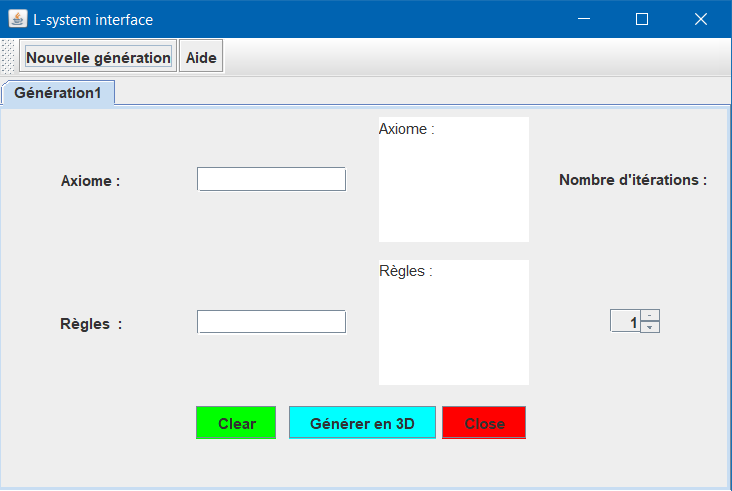
\includegraphics[scale=0.5]{pics/MainFrameGUI.PNG}
    \caption{Fenêtre principale}
    \label{mainframe}
\end{figure}
Il ne vous reste ensuite plus qu'à renseigner votre axiome, ainsi que vos règles et de cliquer sur le bouton \button{Générer en 3D}. Le bouton \button{Close} permet de fermer l'onglet de génération et le bouton \button{Clear} de supprimer votre axiome et vos règles précédemment écrites. Grâce au compteur à droite, vous êtes en mesure de définir le nombre d'itérations de votre génération.

\info{Vous pouvez ouvrir de nouveaux onglets de génération grâce au bouton \button{Nouvelle génération} mais sachez qu'un maximum de trois fenêtres est accepté}

\subsection{Navigation dans l'interface graphique en 3D}
\label{sec:nav_3d}

Pour naviguer dans l'espace 3D, vous pouvez utiliser votre clavier ainsi que votre souris. \info{La souris n'est pas essentielle, le clavier suffit amplement}

\paragraph{Liste des commandes au clavier : }
\begin{itemize}
    \item \textbf{Z} $\xrightarrow{} Avancer$
    \item \textbf{S} $\xrightarrow{} Reculer$
    \item \textbf{Q} $\xrightarrow{} Aller \ à \ gauche$
    \item \textbf{D} $\xrightarrow{} Aller \ à \ droite$
    \item \textbf{A} $\xrightarrow{} Tourner \ la \ caméra \ à \ gauche$
    \item \textbf{E} $\xrightarrow{} Tourner \ la \ caméra \ à \ droite$
    \item \textbf{W} $\xrightarrow{} Prendre \ de \ la \ hauteur$
    \item \textbf{X} $\xrightarrow{} Perde \ de \ la \ hauteur$
    \end{itemize}
\paragraph{Liste des commandes à la souris :}
    \begin{itemize}
    \item \textbf{Mollette Avant} $\xrightarrow{} Zommer$
    \item \textbf{Mollette Arrière} $\xrightarrow{} Dézoomer$
    \item \textbf{Clic Droit} $\xrightarrow{} Maintenir \ puis \ bouger \ la \ souris \ pour \ changer \ l'orientation \ de \ la \ caméra$
    
\end{itemize}

\problem{Vous ne pouvez pas utiliser 2 touches ou plus en même temps pour naviguer. Par exemple, enfoncer les touches \textbf{Z} et \textbf{D} pour aller la direction nord-est  est impossible, il vous faut tourner votre caméra dans la direction où vous voulez aller puis appuyer sur \textbf{Z}.}

Fermez la fenêtre 3D pour pouvoir générer un nouveau L-Systeme sans avoir à rouvrir l'application

\section{Tests de notre logiciel}

\subsection{Exemple test 1}

\subsection{Exemple test 2}

\subsection{Possibles problèmes}

Lorsque vous tentez de générer un L-Système, celui-ci est affiché en 3D en utilisant une méthode récursive, si celui-ci est trop long cela peut entraîner une erreur de type StackOverflowError, la fenêtre 3D restera alors blanche, fermer la puis retenter une génération avec moins d'itérations ou tentez une génération avec d'autres règles.

\section{Mesures de performances}

\section{Possibles améliorations}


	\cleardoublepage
	\pagebreak
	
	\pagenumbering{roman}
	\chapter{Annexes}
	    \section{Sources}
	    \begin{itemize}[label=\textbullet]
	        \item Wikipedia L-Système (EN) : \href{https://en.wikipedia.org/wiki/L-system}{https://en.wikipedia.org/wiki/L-system}
	        \item Wikipedia L-Système (FR) : \href{https://fr.wikipedia.org/wiki/L-Syst\%C3\%A8me}{https://fr.wikipedia.org/wiki/L-Système}
	        \item Developpez.com - Tutoriel Swing :\\
	        \href{https://baptiste-wicht.developpez.com/tutoriels/java/swing/debutant}{https://baptiste-wicht.developpez.com/tutoriels/java/swing/debutant}
	        \item Java doc - Swing
	        \href{https://docs.oracle.com/javase/8/docs/api/javax/swing/JFrame.html}{https://docs.oracle.com/javase/8/docs/api/javax/swing/JFrame.html}
	        \item JOGL : \href{https://jogamp.org/jogl/www/}{https://jogamp.org/jogl/www/}
	        \item Javadoc : \href{https://junit.org/junit4/javadoc/latest/}{https://junit.org/junit4/javadoc/latest/}
	    \end{itemize}
        \section{Remerciements}
		    Triss Jacquiot qui nous a permit de s'inspirer de son rapport pour la mise en forme.
		    
	
\end{document}
